\lstdefinestyle{yaml}{
     basicstyle=\color{red}\footnotesize,
     rulecolor=\color{black},
     string=[s]{'}{'},
     stringstyle=\color{red},
     comment=[l]{:},
     commentstyle=\color{black},
     morecomment=[l]{-}
 }
 \lstset{numbers=left}
 
\chapter{Proof Of Concept} \label{ch:proofOfConcept}

This chapter explores the Proof of Concept (PoC) phase within the context of the thesis, aiming to validate the feasibility and efficacy of implementing SDV technologies. The main objective of this chapter is to translate theoretical concepts into concrete results, demonstrating the practical application of SDV in real-world situations. Through the PoC, we aim to confirm the fundamental principles and features of SDV, including its potential impact on vehicle performance, user experience, and overall safety.

The multifaceted nature of SDV requires a structured approach to its implementation, taking into account factors such as standardized hardware, cloud integration, and over-the-air (OTA) updates. To achieve this, a PoC was designed to address these components individually and holistically, ensuring a seamless integration that aligns with the envisioned paradigm shift in automotive manufacturing. Furthermore, this chapter aims to demonstrate the collaborative efforts with industry-leading technologies and platforms, highlighting the strategic partnerships forged with key players in the automotive and software development sectors. By aligning with renowned entities, the PoC aims to leverage their expertise, technologies, and frameworks, thereby enhancing the robustness and scalability of the SDV ecosystem.

Test and Validation are the concluding phases of this chapter, where the Proof of Concept is subjected to real-world scenarios. A demonstration involving a Raspberry Pi (RPi) serves as a tangible validation of the implemented SDV functionalities. This section serves as the litmus test, affirming the seamless orchestration of SDV within the envisioned architecture.

The exploration of the POC begins by detailing the services and technologies offered by Amazon Web Services (AWS) in the IoT, data management, and automotive essential for project implementation.

\section{AWS Used Services}
As discussed in previous chapters, the development of SDV technology requires a cloud infrastructure to handle server-side operations. AWS is a leading player in the cloud world, and therefore an ideal alternative for the advancement of SDV, as well as an active partner in the implementation of technologies that contribute to the creation of a publicly available SDV for all. The following discussion introduces and analyzes, via AWS documentation the key tools for successful Proof of Concept (POC) implementation.

\begin{itemize}
    \item AWS CLI: The AWS Command Line Interface (CLI) is an essential tool for developing with AWS services. t allows interaction with AWS services from the command line of a local PC, enabling the creation of infrastructure and management of properties from the command line.
    \item AWS Boto: Boto is an AWS SDK made for Python. A software Development Kit (SDK), more generally, is a set of creation tools specifically for developing and running software in a single platform. It includes resources such as documentation, examples, and APIs to facilitate faster application development. Boto basically works as an interface for applications that need to interact with and take advantage of the services provided by AWS. The AWS SDK for JavaScript v3 is another example of an SDK for JavaScript that works basically in the same way.
    \begin{figure}[h]  % 'h' significa che la figura viene posizionata qui
        \centering
        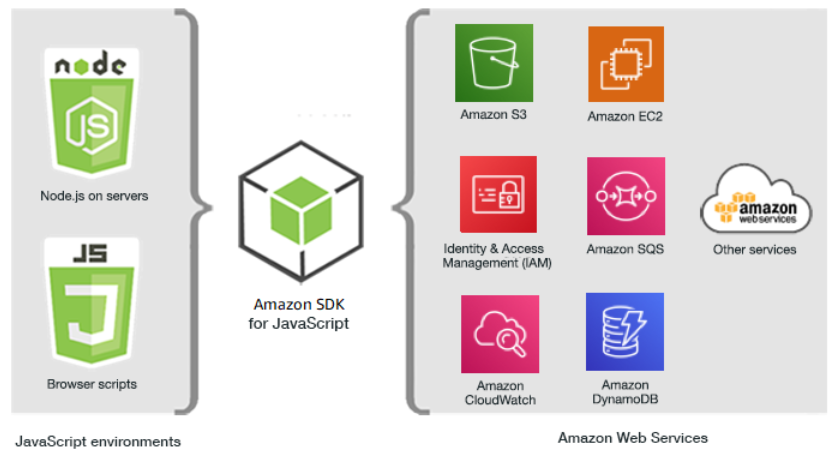
\includegraphics[width=0.8\textwidth]{images/AWSSDK.png}  % Sostituisci 'nome_immagine' con il nome del tuo file immagine e l'estensione
        \caption{The high level rappresentation of the AWS SDK for JavaScript v3 \cite{AWSSDK}}
        \label{fig:AWSSDK}
    \end{figure}
    \item AWS CDK: The AWS Cloud Development Kit (CDK) "is an open-source software development framework for defining cloud infrastructure in code and provisioning it through AWS CloudFormation" \cite{WhatIsTheAWSCDK}. This tool was used in the final phase of the POC design to automate the creation of the stack comprising all the services used.
    \item AWS IoT Core: AWS IoT Core provides the ability to connect IoT devices to AWS cloud services. AWS IoT Core enables the connection of IoT devices to AWS cloud services. It simplifies the integration of IoT devices with other AWS services. This is especially relevant in the automotive industry, where vehicle system ECUs can be viewed as multiple IoT devices. Communication between the device and AWS services can occur in several modes, with the MQTT protocol being the most important for this project. The device can be connected by developing applications that utilize the SDK libraries. Once the data is transmitted, it can be utilized for various purposes such as testing, validation, and analysis.
    \begin{figure}[h]  % 'h' significa che la figura viene posizionata qui
        \centering
        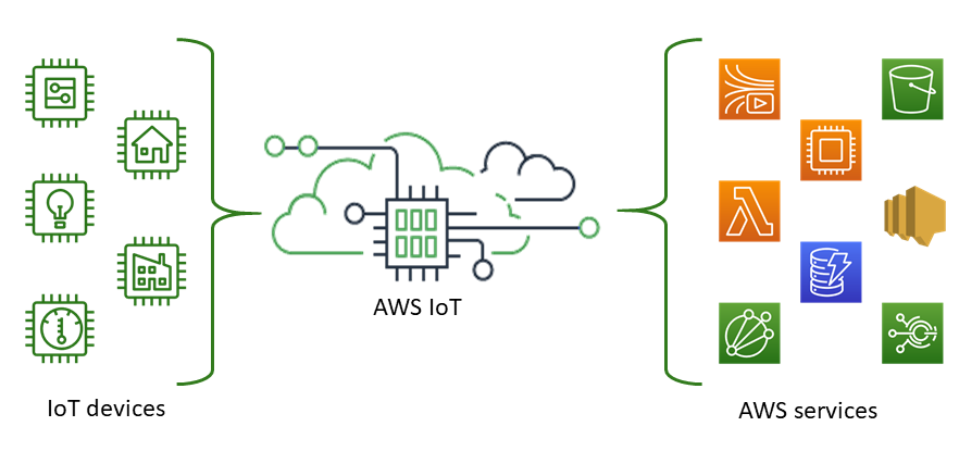
\includegraphics[width=0.8\textwidth]{images/AWSIoTCore.png}  % Sostituisci 'nome_immagine' con il nome del tuo file immagine e l'estensione
        \caption{AWS IoT Core connection system beetween IoT device and AWS service \cite{AWSIoTCore}}
        \label{fig:AWSIoTCore}
    \end{figure}
    \item AWS IoT Greengrass: "AWS IoT Greengrass is an open source Internet of Things (IoT) edge runtime and cloud service that helps you build, deploy and manage IoT applications on devices" \cite{AWSIoTGreengrass}. It is designed to work with intermittent connections and can manage fleets of devices in the field, locally or remotely, using MQTT or other protocols. Once installed, this service can be accessed through the command line. It was utilized in the early stages of project development as an agent to handle updates on the vehicle simulator side. However, this solution will be replaced by a custom solution as explained later.
    \item AWS IAM: "AWS Identity and Access Management (IAM) is a web service for securely controlling access to AWS services [...] such as access keys, and permissions that control which AWS resources users and applications can access" \cite{AWSIAM}. IAM is a service that provides a powerful access management mechanism. However, for the purpose of this thesis, only the relevant functionality to the project will be analyzed, specifically IAM's role management capabilities.An IAM role is an identity within AWS that can be assigned specific permissions via permission policies to determine what actions can and cannot be taken. Roles can be assumed by users, applications, or services that do not normally have access to the specific AWS resources. The IAM service also provides another important concept, that of policy, which is an AWS object that, when attached to an identity (including roles) or a resource, enables the creation of permissions and access control to other resources. For example, as explained below, a policy can be attached to the cloud representation of an IoT Core device to enable the connection of the physical dual IoT device or to grant Subscriber or Publisher permissions in a communication via MQTT protocol.
    \item AWS Lambda: AWS Lambda is a computing service that provides the ability to run code without servers. It runs code on a high-performance computing infrastructure and handles administrative tasks related to computing resources autonomously, such as server and operating system management, capacity provisioning, automatic scaling, and logging. It is possible to run code for potentially any type of backend application or service \cite{AWSLambda}. Code can be written directly in Lambda console or imported from the local environment, and it supports several languages, including Python and JavaScript. The Lambda service can also manipulate data from other AWS services or manage tasks with services outside AWS as will be analyzed below.
    \item AWS Codepipeline: AWS CodePipeline is a fully managed continuous delivery service that automates release pipelines for software updates. It enables fast and reliable updates to applications and infrastructure, facilitating the rapid release of new features, iterative development based on feedback, and bug detection through testing every code change. The software release process can be modeled and configured quickly via the stages execution. A stage is a logical unit that creates an isolated environment and allows for the execution of a limited number of concurrent software changes. Each stage contains actions that are executed on application artifacts, such as source code from Codecommit. For instance, as shown in the image \ref{fig:AWSCodepipeline}, it is feasible to establish a software development pipeline that incorporates a codecommit repository as its source stage. This way, a codecommit-related event triggers the pipeline execution which then proceeds to the software build stage. An execution is defined as a series of modifications released from a pipeline.   Each execution represents a set of modifications, such as a merged commit or a manual release of the last commit. Subsequently, the pipeline moves on to the test stage where the desired tests can be launched via Codebuild, and finally delivers the application for production. 
    \begin{figure}[h]  % 'h' significa che la figura viene posizionata qui
        \centering
        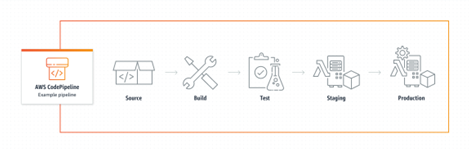
\includegraphics[width=0.8\textwidth]{images/AWSCodepipeline.png}  % Sostituisci 'nome_immagine' con il nome del tuo file immagine e l'estensione
        \caption{An example of a CodePipeline in which some stages are reported \cite{AWSCodepipeline}}
        \label{fig:AWSCodepipeline}
    \end{figure}
    \item AWS Codebuild: AWS CodeBuild is a fully managed build service in the cloud that provides source code compilation, unit testing, and production of executable programs ready for distribution \cite{AWSCodebuild}. CodeBuild provides out-of-the-box configuration of compilation environments for popular programming languages, such as Python. It is also possible to create build platforms for programming languages for which there is no preconfiguration, but in this case it is necessary to leverage multiple AWS services. It is also possible to use codebuild to run tests on application code using for example the pytest tool that allows you to test python code.
    \item AWS Codecommit: "AWS CodeCommit is a version control service that enables you to privately store and manage Git repositories in the AWS Cloud" \cite{AWSCodecommit}. This service becomes particularly interesting in the context of multiple services working together, including Lambda, Codepipeline, and Codebuild, because it allows the repository's Git and all its associated events (such as commit and push) to be used to trigger events that can automate various operations, such as triggering a pipeline in Codepipeline. As a result, CodePipelines typically use a CodeCommit repository as their inputo Source stage.
    \item Amazon S3: "Amazon Simple Storage Service (Amazon S3) is an object storage service that offers industry-leading scalability, data availability, security, and performance" \cite{AWSamazonS3}. The data saved in the storage is physically placed in multiple locations to ensure the durability of the data even if there is tampering with an item due to the presence of these copies; optionally, it can also be chosen to store the data in a single location to reduce the cost of the service. Amazon S3 can be used for data collection, aggregation, and analysis in many contexts and scenarios, but in the scope of this project, this service is used to store data that is transferred from one stage of the Codepipeline to another. Amazon's Codepipeline service automatically implements this method of output use. However, data stored in S3 from one stage to another can be manipulated through integration with other AWS services, such as Lambda.
    \begin{figure}[h]  % 'h' significa che la figura viene posizionata qui
        \centering
        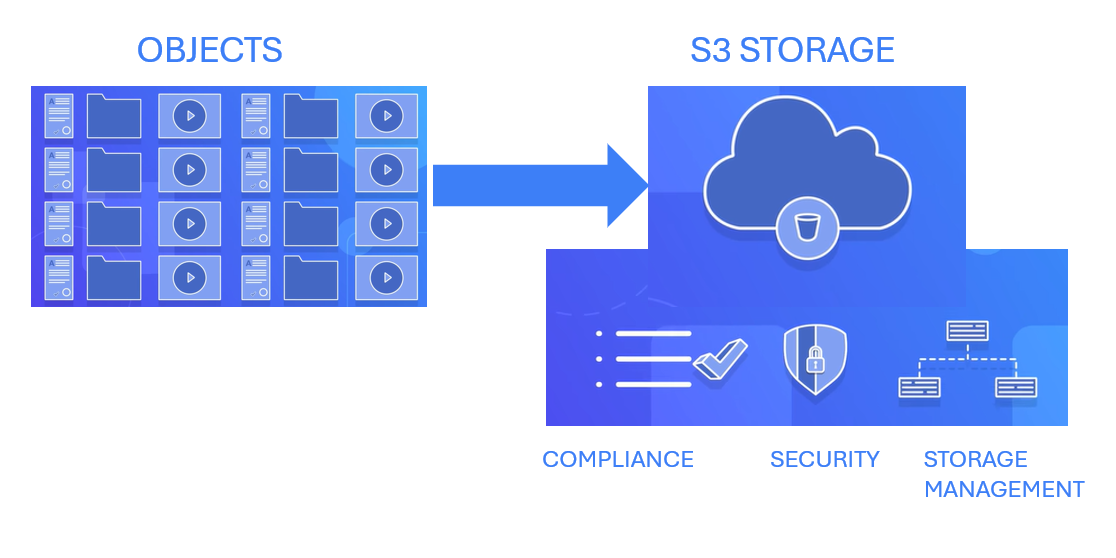
\includegraphics[width=0.8\textwidth]{images/AWSS3.png}  % Sostituisci 'nome_immagine' con il nome del tuo file immagine e l'estensione
        \caption{Amazon S3 high level storing rappresentation}
        \label{fig:AWSS3}
    \end{figure}
    \item Amazon ECR: "Amazon Elastic Container Registry (Amazon ECR) is an AWS managed container image registry service that is secure, scalable, and reliable. Amazon ECR supports private repositories with resource-based permissions using AWS IAM. This is so that specified users or Amazon EC2 instances can access [...] container repositories and images" \cite{AmazonECR}. Basically, as shown in the figure \ref{fig:AWSECR}, once the software has been produced and packaged, for example through the use of the CodeBuild service, it can be uploaded to Amazon ECR. The ECR takes care of encrypting the image and controlling access to it, and then automatically manages the entire lifecycle of the image. Once the image is on ECR, it can be used either as an image for local download or through other AWS services. 
    \begin{figure}[h]  % 'h' significa che la figura viene posizionata qui
        \centering
        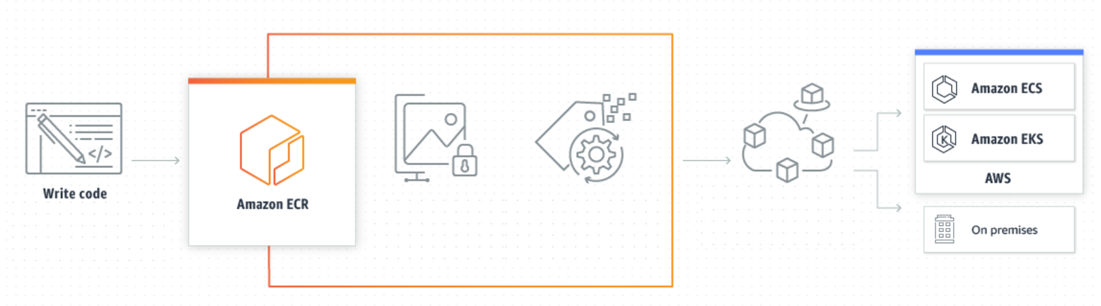
\includegraphics[width=0.8\textwidth]{images/AWSECR.png}  % Sostituisci 'nome_immagine' con il nome del tuo file immagine e l'estensione
        \caption{Example of how Amazon ECR works in production and for pulling images \cite{AWSECR}}
        \label{fig:AWSECR}
    \end{figure}
    \item EC2: Amazon Elastic Compute Cloud (Amazon EC2) provides scalable, on-demand computing capacity in the Amazon Web Services (AWS) cloud. With Amazon EC2, users can create and use virtual machines in the cloud, instantiating resources as needed to perform compute operations. Amazon EC2 is a common choice for rapidly deploying applications because it provides an excellent computing resource at a low cost \cite{AWSEC2}, and it is possible to manage networks of different instances of EC2 virtual machines through Amazon Virtual Private Cloud (VPC) and set their relative security, either on a per-instance basis or on an overall network basis. Additionally, it is possible to increase the capacity (scale up) of the instance after creation to handle computationally heavy tasks, such as spikes in website traffic. Conversely, if utilization decreases, capacity can be reduced (scale down). EC2 instances can be launched with Amazon Machine Images (AMIs), which are preconfigured templates containing the necessary components to use the server, including the operating system and additional software. AWS provides pre-built AMIs, but it is also possible to create your own AMIs using containers. Furthermore, it is possible to connect to an EC2 instance through various communication systems, such as using SSH keys provided at the time of instance creation.
    \item AWS System Manager: AWS Systems Manager is a service that provides visibility and control of the infrastructure on AWS.  It allows users to view operational data from multiple AWS services and manage the automation of operational tasks across different AWS resources \cite{AWSSM}. The AWS System Manager service is particularly relevant to the project due to its application management capability, namely the Parameter Store. Parameter Store is used to securely store configuration data and secrets, such as passwords, connection strings, and Amazon Machine Image (AMI) identifiers. Values are stored hierarchically by assigning hierarchical names to stored values using the "/" character, while maintaining the uniqueness of the name. For example, names such as Parameters/Parameter1, Parameters/Parameter2 can be used. In addition, it is possible to choose whether to store the data as plain text or encrypted data. Stored data can be retrieved directly from other services, for example, by interacting with Lambdas and SDK code functions.
    \item Amazon Kinesis Data Streams: Amazon Kinesis Data Streams is used to collect and process large streams of data records in real time, and eventually route them through other AWS services to various data collection and analysis applications, such as Amazon S3 as it is shown in the image \ref{fig:AmazonKinesis}. "The delay between the time a record is put into the stream and the time it can be retrieved (put-to-get delay) is typically less than 1 second. In other words, a Kinesis Data Streams application can start consuming the data from the stream almost immediately after the data is added" \cite{AWSKinesis}.
    \begin{figure}[h]  % 'h' significa che la figura viene posizionata qui
        \centering
        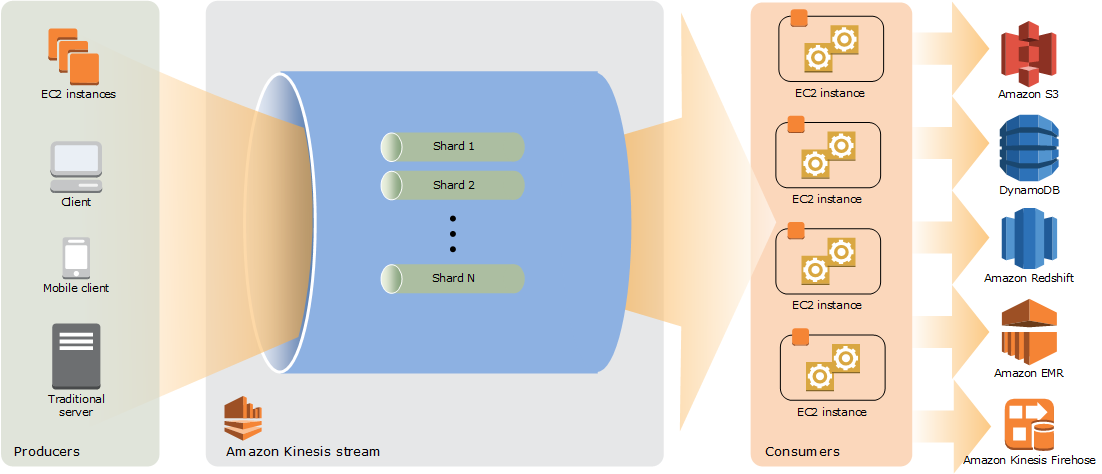
\includegraphics[width=0.8\textwidth]{images/AmazonKinesis.png}  % Sostituisci 'nome_immagine' con il nome del tuo file immagine e l'estensione
        \caption{Illustration of the high-level architecture of Kinesis Data Streams with some examples of services that use the output of the stream. \cite{AmazonKinesis}}
        \label{fig:AmazonKinesis}
    \end{figure}
    \item Amazon Timestream: Amazon Timestream is a time-series database that allows you to store and easily analyze large amounts of data stored at regular intervals, ensuring that the time-series data is always encrypted, whether at rest or in transit. This service simplifies the complex process of managing the lifecycle of data by providing storage tiering with an in-memory store for current data and a magnetic store for historical data using Amazon S3 space. The transition of data between these two storage types is enabled through the use of user-configurable policies. The data lifecycle management mechanism makes Amazon Timestream ideal for handling telemetry data from IoT devices, for example. The service also provides a built-in interface for accessing data through a query engine \cite{AWSTimestream}. The Timestrem service also provides an interface for Grafana to view and analyze stored data, which will be explored later.
    \item DinamoDB: Amazon DynamoDB is a full-featured NoSQL database service that provides high perfomances both speed and scalability. DynamoDB removes the administrative complexity of running and scaling your distributed database, so there's no need to manage provisioning, hardware setup and configuration, replication, software patching, or cluster sizing. DynamoDB also provides encryption at rest, eliminating the operational costs associated with protecting sensitive data. DynamoDB provides the ability to change the allocation of resources needed to store data in real time to use only the resources required. Additionally, DynamoDB offers on-demand backup functionality for long-term retention and archival purposes, as well as point-in-time recovery to safeguard against accidental write or delete operations. This feature enables users to restore a table to any point within the last 35 days \cite{AWSDynamoDB}. Note that this service was not utilized in the final version of the project, but was considered during development as an alternative for data storage and as a case study for understanding the data storage mechanisms used by AWS services.
    \item Amazon Cloudwatch: Amazon CloudWatch is a system to monitor the Amazon Web Services (AWS) resources and the applications running on the infrastructure in real time. With the use of CloudWatch it is possible to collect and track metrics from other AWS services such as Lambda, which are numeric variables that can be measured and analyzed for resources applications \cite{AWSCloudwatch}. Practically this service represents the center for viewing and analyzing logs from the various AWS services in use.
\end{itemize}

All of the previously listed services have been useful, both as an active part in the project's realization and as potential options for the project's implementation, which will be analyzed below. The analysis of the POC will start with a description of the project's design, followed by an analysis of how the various services are actively involved in the project, and then an analysis of the interaction between the various elements that make up the architecture.

\section{Architectural design}
This section delves into the heart of the project implementation, starting with a high-level view of the various systems that make up its realization and transitioning to a visualization of the interactions between the various elements.

The study and analysis of the Software Defined Vehicle case study revealed that three fundamental elements were essential to create a concrete example of SDV implementation:
\begin{itemize}
    \item TCU simulator: The TCU simulator is a system that replicates the basic functions of a telematic control unit (TCU). The system has the capability to send data packets and receive updates from a cloud server structure.
    \item Cloud infrastructure: The cloud infrastructure must be capable of managing both the data from the TCU and the update function.
    \item Data viewer:  The data viewer is a platform that enables the visualization of manipulated and processed data in a manner that clearly displays changes in data behavior resulting from variations in the data and updates to the TCU.
\end{itemize}

With these three elements, a practical implementation made it possible to achieve what should happen in an SDV: having a vehicle system capable of updating itself via Over The Air updates. To support this implementation, it was necessary to use the services previously mentioned for creating the cloud infrastructure through the services made available by AWS.

Now, let's look at the components of the POC in detail through a high-level architectural representation of the previously introduced elements and a more detailed analysis of the code that compose them.

\subsection{TCU Simulator}
This project considers a Telematics Control Unit (TCU) to be a hardware system capable of generating data from one or more subsystems of a potential vehicle, collecting it, and then preparing it for transmission outside the vehicle. To familiarize with this structure and to design the sample project, it was necessary to simulate a TCU in a way that was as close as possible to a real system, without having the availability of a real vehicle. Therefore, to simplify the concept, a Raspberry Pi board was chosen as the TCU endpoint capable of generating telemetric data.

\begin{figure}[h]  % 'h' significa che la figura viene posizionata qui
    \centering
    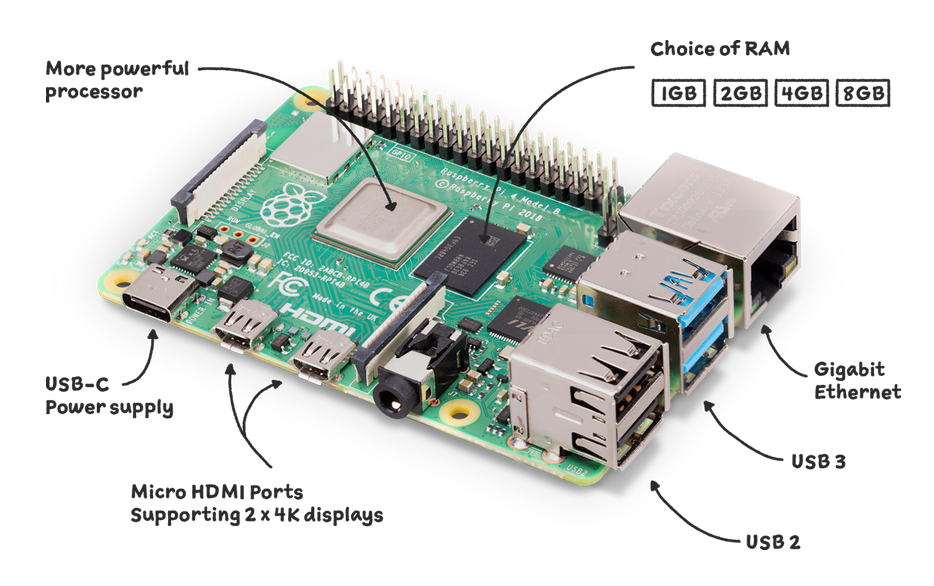
\includegraphics[width=0.8\textwidth]{images/raspberrypi.png}  % Sostituisci 'nome_immagine' con il nome del tuo file immagine e l'estensione
    \caption{Illustration of a RaspberryPi board with its periferics \cite{raspberrypi}}
    \label{fig:raspberrypi}
\end{figure}

As shown in the figure above \ref{fig:raspberrypi} a RaspberryPi is a board containing everything necessary to function as an independent system to which various peripherals can be attached, making it the ideal abstraction of a general-purpose TCU needed to implement the SDV SOC case study.
Before working with the raspberry, it was necessary to implement the project on a virtual machine, which greatly facilitated the development and testing of the written code on a PC with a different operating system and architecture than the RaspberryPi board.

The simulator was thought to consist of four different software components, each with its own functionality, during its various stages of development:
\begin{itemize}
    \item A component is responsible for connecting to the cloud server to send telematics data;
    \item A component for establishing a connection to the cloud server in order to update the telematics unit;
    \item A component for generating telematics data;
    \item A component for recognizing and managing local unit updates.
\end{itemize}
An external script manages the startup of the simulation unit via command line using the four items. 

Analyzing these four elements in detail, the first element in chronological order was the component responsible for connecting the system to the cloud infrastructure via the MQTT protocol. This component required the presence of an active cloud-side IoT Core service, which, as we will discuss later, generates a certificate with an attached public and private key pair to ensure the device's identity. The consideration of the cloud infrastructure will be analyzed later when the cloud infrastructure is discussed.

In order to establish a connection to the cloud platform, the following code snippet from listing \ref{lst:MQTTConnection} is analyzed. The Python script launches and establishes a connection to the IoT Core server using the function specified on line 1 from the designated library. This enables the data to be sent to the server. The code on line 12 creates an MQTT client. On line 13, the code configures the client's host name and port number. Finally, on line 14, the code is configured with the authentication certificates. It is important to note that these files are stored locally on the device and must be accessed by the linking script. The MQTT connection will be established on the topic specified on line 19. This will enable the AWS service, which will be connected to the topic through appropriate policies (as we will see later), to receive the transmitted data.

\begin{lstlisting}[language=Python, caption={MQTT connection to the IoT Core AWS service}, label=lst:MQTTConnection, linerange={1-23}]
from AWSIoTPythonSDK.MQTTLib import AWSIoTMQTTClient
certificate_path="./Permanent/Certificates/"
def telemetry_handler():
    global mqttc
    global connection_event
    VIN = "HawkbitDevice001"  ##This is the Thing name
    ENDPOINT = "**********.amazonaws.com" #This field contains the aws region
    CERT_FILEPATH = f"{certificate_path}{VIN}.cert.pem"
    PRIVATE_KEY_FILEPATH = f"{certificate_path}{VIN}.private.key"
    ROOT_CA_FILEPATH = f"{certificate_path}root-CA.crt"
    mqttc = AWSIoTMQTTClient(VIN)
    mqttc.configureEndpoint(ENDPOINT, 8883)
    mqttc.configureCredentials(ROOT_CA_FILEPATH, PRIVATE_KEY_FILEPATH, CERT_FILEPATH)
    if mqttc.connect():
        print("Connected to IoT core. Now the device sends its telemetry every 1 seconds")
        connection_event.set() #Send connected signal to the main
        publish_topic = f"device/{VIN}/telemetry"
\end{lstlisting}

The second item of analysis used in the realization of the simulator is the component that allows connecting to the OTA server to detect and download OTA updates. This was made possible by utilizing the 'Device Simulator' provided by Hawkbit. The simulator is a Java script that takes advantage of the Hawkbit Server interface to connect to the server and listen for updates specifically targeted to the device.

The code automatically establishes the connection when started through the simulation properties. For experimental design purposes, the device name is set statically as shown on line 2 of code fragment \ref{lst:SimulationPropertiesHDS}, while the server's IP address to connect to is taken as input in the provided code \ref{lst:ArgumentsHDS}, as shown on line 6.

\begin{lstlisting}[language=Java, caption={Simulation properties of the Hawkbit Device Simulator}, label=lst:SimulationPropertiesHDS]
public static class Autostart {
    private String name = "HawkbitDevice001";
    private int amount = 1;
    @NotEmpty
    private String tenant = "DEFAULT";
    private Protocol api = Protocol.DMF_AMQP;
    private String endpoint = "http://localhost:8080";
    private int pollDelay = (int) TimeUnit.MINUTES.toSeconds(30);
    private String gatewayToken = "";
    ...
}
\end{lstlisting}

\lstset{numbers=left}
\begin{lstlisting}[language=Java, caption={Input arguments to set the ip of the OTA server to contact}, label=lst:ArgumentsHDS]
public static void main(final String[] args) {
    //take endpoint rabbit server as input
    if (args.length > 0) {
        String newHost = args[0];
        if (!newHost.isEmpty()) {
            System.setProperty("spring.rabbitmq.host", newHost);
        }
    }
    SpringApplication.run(DeviceSimulator.class, args);
}
\end{lstlisting}

As demonstrated in the relevant sections of source code \ref{lst:OverallReadHDS}, when the device receives a download signal, it performs a series of security checks before starting to download the received data into the folder specified in line 4 of the code, using a stream that takes the incoming data from the link and places it in the selected folder, with the filename obtained from the download URL.

\begin{lstlisting}[language=Java, caption={Downloading files from the OTA server to the specific device simulator folder}, label=lst:OverallReadHDS]
private static long getOverallRead(final CloseableHttpResponse response, final MessageDigest md, final String url) throws IOException {
    long overallread = 0L;
    String[] urlParts = url.split("/");
    File downloadFolder = new File("./TCU/downloads");
    if (!downloadFolder.exists()) { //If "Download" folder doesn't exist
        boolean created = downloadFolder.mkdirs();
        if (!created) {
            System.err.println("Error in the directory creation!");
        }
    }
    File downloadFile = new File("./TCU/downloads/"+urlParts[10]);
    try (FileOutputStream outputStream = new FileOutputStream(downloadFile);
    final BufferedOutputStream bos = new BufferedOutputStream(new DigestOutputStream(outputStream, md))) {
        try (BufferedInputStream bis = new BufferedInputStream(response.getEntity().getContent())) {
            byte[] buffer = new byte[8192]; //byte dimension from createBuffer of ByteStream.class
            int bytesRead;
            while ((bytesRead = bis.read(buffer)) != -1) {
                bos.write(buffer, 0, bytesRead); //Here only for the md hash correctness.
                overallread += bytesRead;
            }
        }
    }
    return overallread;
}
\end{lstlisting}

During the TCU software update phase, at the time the server sends the update, the device in charge of listening for the update receives the update signal and the update download, the log file is written. The file is created in a specially created location each time the system is booted, or it is overwritten if it already exists. It will print a confirmation if the download was successful \ref{fig:update_log_HDS}, and the cause of the error if the download was unsuccessful.

\begin{figure}[h]  % 'h' significa che la figura viene posizionata qui
    \centering
    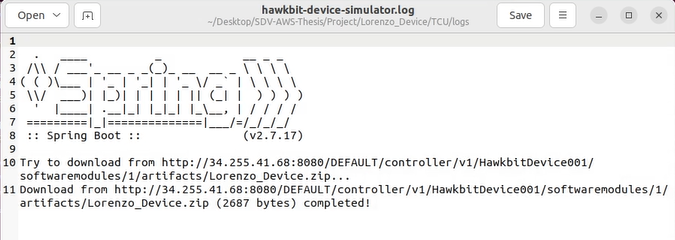
\includegraphics[width=0.8\textwidth]{images/update_log_HDS.png}  % Sostituisci 'nome_immagine' con il nome del tuo file immagine e l'estensione
    \caption{Update log file of the Device Simulator}
    \label{fig:update_log_HDS}
\end{figure} 

The third component of the simulator is the heart of the TCU, which is the system that can generate the simulated vehicle data that changes in a progressive manner over time. This component has undergone several modifications during the course of development, in particular it was initially designed as a command line interface device written in Python language.

More specifically, as shown in Figure \ref{fig:telemetryV1}, in the first version of the simulator, once started, based on commands given by the user via the command line, it was able to increase or decrease its "speed" to a limit until it stopped. The speed information, which varied over time, was sent every second to the component that manages communication with the IoT Core server and then sent to the server.

\begin{figure}[h]  % 'h' significa che la figura viene posizionata qui
    \centering
    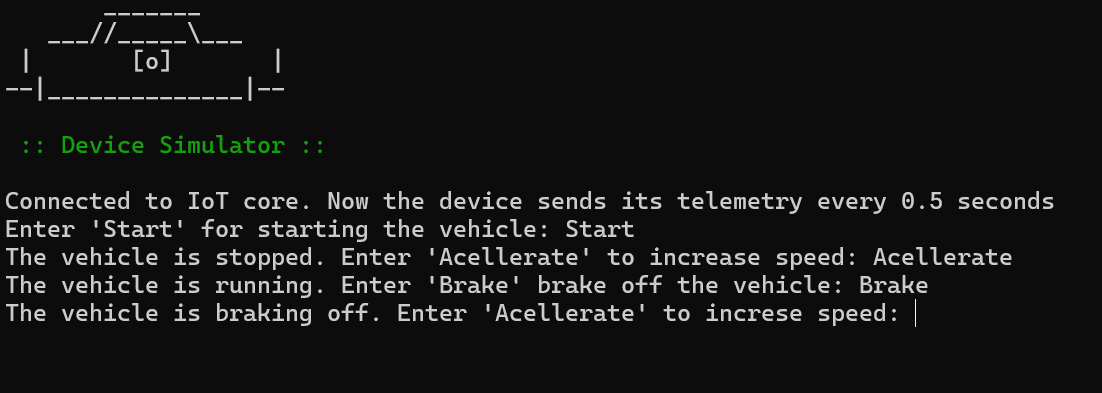
\includegraphics[width=0.8\textwidth]{images/telemetryV1.png}  % Sostituisci 'nome_immagine' con il nome del tuo file immagine e l'estensione
    \caption{A snapshot of the first version of the TCU interface}
    \label{fig:telemetryV1}
\end{figure} 

In this case, there were two different versions of the speed handler code: the first one represented the initial state of the simulated vehicle, while the second one represented the vehicle after the update. In this way, it was clear that the update of the vehicle had occurred.

At a later stage, for the creation of the final Python TCU, it was decided to increase the number of telemetry data provided in such a way as to be able to collect and analyze a more realistic number of values in the cloud, but at the expense of a predefined data generation not decided by the user. This solution solved the fact that a real TCU would not present a graphical interface, but would simply collect the data generated by the subsystems present in the vehicle as a function of time. In this case, it was possible to build five subsystems capable of generating data every second in a way that can be considered as close as possible to a real system, then this data is collected by an orchestrating script \ref{lst:TCUOrchestrator} that aggregates it to make it ready to be sent to the listening cloud service.
\begin{lstlisting}[language=Python, caption={TCU orchestrator that collects data from other subsystems}, label=lst:TCUOrchestrator]
for sub in subsystems:
    values[sub.get_name()] = sub.get_info(t)
    values["Timestamp"] = datetime.isoformat(datetime.utcnow())
    values["DeviceID"] = f"{VIN}"
    print(values)
    messageFinal=json.dumps(values)
    mqttc.publish(publish_topic, messageFinal, 0)    
\end{lstlisting}

As shown in code \ref{lst:TCUOrchestrator}, an iteration is performed on each subsystem present in the simulator, the data is collected in Json format and sent to the AWS IoT Core service through the previously seen object in script \ref{lst:MQTTConnection} to establish the connection with the service itself. This system allows you to have maximum modularity of the subsystems, therefore possibly being able to add new ones with future updates, the only constraint is to specify the list of present subsystems in the Python init \ref{lst:TCUInit} file and then add any new subsystems present.
\begin{lstlisting}[language=Python, caption={TCU init file for the import of the TCU subsystems}, label=lst:TCUInit]
from .airConditioning import AirConditioning
from .airbag import Airbag
from .heatedSeats import HeatedSeats
from .abs import ABS
from .engine import Engine
from .battery import Battery
subsystems = [Engine(), Battery(), AirConditioning(), Airbag(), HeatedSeats(), ABS()]  
\end{lstlisting}

Now, we will examine one of the sample subsystems developed for the project and assess its primary functions. A simulator has been implemented to generate data from a hypothetical vehicle battery in the case of hybrid or fully electric vehicles. This subsystem reports three main pieces of information: the energy added to the battery through regenerative braking, the total energy stored in the battery at a given moment, and the battery temperature at a given instant. The vehicle is considered a system where an electric motor provides energy during acceleration, causing a decrease in the battery's energy. During deceleration, part of the energy is stored in the battery through regenerative braking. The battery's temperature varies over time due to these operations.

The functions listed in code block \ref{lst:BatterySubsystem} are the most important parts of the class composing the subsystem simulator. These functions practically identify the common parts of each subsystem present in the project. The telemetry data is first aggregated in a JSON format and then returned by these functions. Additionally, a function is required to return an identifying name of the subsystem. This name is useful to the orchestrator shown previously in \ref{lst:TCUOrchestrator} at line 2 for constructing the data packet to be sent to the server correctly.
\begin{lstlisting}[language=Python, caption={Battery subsystem return code}, label=lst:BatterySubsystem]
def get_info(self, time):
    return {
        "StateOfCharge" : self.stateOfCharge,
        "BatteryTemperature": self.batteryTemperature,
        "EnergyAdded" : self.energyAdded,
    }
def get_name(self):
    return "Battery"  
\end{lstlisting}
During the updating phase, this data \ref{fig:TCUsimulatorP}, as well as all other subsystems, is created using a different algorithm. This ensures that when the telemetry data is analyzed, the download event is clearly visible. It is important to note that each Python subsystem has a related set of tests that can be utilized by the cloud structure, as analyzed further below.
\begin{figure}[h]  % 'h' significa che la figura viene posizionata qui
    \centering
    \includegraphics[width=0.8\textwidth]{images/TCUsimulatorP.png}  % Sostituisci 'nome_immagine' con il nome del tuo file immagine e l'estensione
    \caption{A snapshot of the TCU simulator on the virtual machine}
    \label{fig:TCUsimulatorP}
\end{figure}

In the final phase of the project, it was decided to modify the simulator to use a compiled script. This change makes the system more similar to a real world situation, since in a real environment there would be systems where it is not possible to have scripts based on interpreters such as the Python language, for reasons of size and resources, but where compiled programs are needed, which are more optimized. In order to do so and to give a concrete demonstration of the changes made to the infrastructure as analyzed in the following, it was decided to create a much simpler TCU simulator in C language (C simulator code). 
\begin{figure}[h]  % 'h' significa che la figura viene posizionata qui
    \centering
    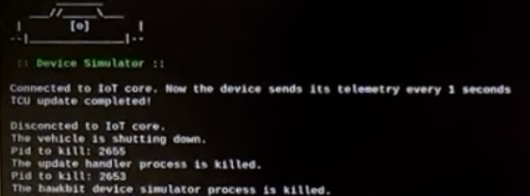
\includegraphics[width=0.8\textwidth]{images/TCUsimulatorC.png}  % Sostituisci 'nome_immagine' con il nome del tuo file immagine e l'estensione
    \caption{A snapshot of the TCU compiled simulator on the Raspberry Pi interface}
    \label{fig:TCUsimulatorC}
\end{figure}

In order to be compatible with both the first and second versions of the simulator (for backward compatibility), it was also necessary to adapt the orchestrator element \ref{lst:TCUOrchestrator} to be capable of recognizing the type of simulator to which it would be interfaced with. To make this possible, a specification file indicating the type of simulator used \ref{lst:TCUManifest} was added to each TCU simulator.
\begin{lstlisting}[language=c, caption={Manifest example of compiled TCU simulator}, label=lst:TCUManifest]
<?xml version="1.0" encoding="UTF-8" standalone="yes"?>
<project>
    <name>C Project</name>
    <language>C</language>
    <compiler>gcc</compiler>
    <build_command>gcc main.c -o main.exe</build_command>
    <run_command>./main.exe</run_command>
</project>
\end{lstlisting}


\subsection{Cloud Infrastructure}
\subsection{Data Viewer}

\section{Test and Validation}
\subsection{RPi demo}